%==============================================================================
% USF — Unit-Streamed Fine-Tuning. Artículo 1 (el sistema de streaming).
% Formato IEEE (revista). Versión en español de main.tex.
% REGLA: todo número de este artículo está medido. Sin marcadores de posición.
%==============================================================================
\documentclass[journal]{IEEEtran}

\usepackage[T1]{fontenc}
\usepackage[utf8]{inputenc}
% es-tabla: babel rotula las tablas «Cuadro» por defecto; en español técnico se usa
% «Tabla», y además debe concordar con el \crefname{table} de más abajo.
\usepackage[spanish,es-noquoting,es-nodecimaldot,es-tabla]{babel}
\usepackage{graphicx}
\usepackage{booktabs}
\usepackage{amsmath,amssymb,amsthm}
\usepackage{mathtools}
\usepackage{algorithm}
\usepackage{algpseudocode}
\usepackage{enumitem}
\usepackage{xcolor}
\usepackage{tikz}
\usetikzlibrary{arrows.meta}
\usepackage[hidelinks]{hyperref}
\usepackage{cleveref}

% Paleta de la Fig. 1: una visita o paga lectura de disco, o encuentra la unidad residente.
\definecolor{ioload}{RGB}{178,24,43}
\definecolor{iohit}{RGB}{33,102,172}

% --- entornos de teoremas en español -----------------------------------------
\newtheorem{theorem}{Teorema}
\newtheorem{corollary}[theorem]{Corolario}
\newtheorem{proposition}[theorem]{Proposición}
\newtheorem{definition}[theorem]{Definición}
\newtheorem{remark}[theorem]{Observación}

% cleveref en español
\crefname{theorem}{Teorema}{Teoremas}
\crefname{corollary}{Corolario}{Corolarios}
\crefname{proposition}{Proposición}{Proposiciones}
\crefname{definition}{Definición}{Definiciones}
\crefname{remark}{Observación}{Observaciones}
\crefname{table}{Tabla}{Tablas}
\crefname{algorithm}{Algoritmo}{Algoritmos}
\crefname{section}{Sección}{Secciones}
\crefname{equation}{Ecuación}{Ecuaciones}
% Sin esto cleveref escribe «Figure» y contradice el pie, que babel rotula «Figura».
\crefname{figure}{Figura}{Figuras}
\Crefname{figure}{Figura}{Figuras}

% algorithmicx en español
\renewcommand{\algorithmicfor}{\textbf{para}}
\renewcommand{\algorithmicdo}{\textbf{hacer}}
\renewcommand{\algorithmicend}{\textbf{fin}}
\floatname{algorithm}{Algoritmo}

% IEEEtran fija «Proof» en su propio macro; babel no lo alcanza.
\renewcommand{\IEEEproofname}{Demostración}

\newcommand{\usf}{USF}
\newcommand{\VJP}{\mathrm{VJP}}
\newcommand{\Wu}{\lvert W_u \rvert}
\newcommand{\sthree}{S\textsuperscript{3}}

\begin{document}

% El título se mantiene en inglés a propósito: el acrónimo USF deriva de «Unit-Streamed
% Fine-Tuning», y traducirlo lo dejaría huérfano («Ajuste Fino por Streaming de Unidades» daría
% AFSU). El nombre del método es un nombre propio y no se traduce, igual que LoRA o QLoRA.
% Sin \\ manual: IEEEtran centra y equilibra el título mejor que un salto forzado.
\title{\usf{}: Unit-Streamed Fine-Tuning of Large Language Models with Exact Gradients on
Consumer GPUs}

\author{
Nicolas Andrey Orozco Giraldo, Luis Eduardo Muñoz Guerrero\\
\textit{Universidad Tecnológica de Pereira}\\
Pereira, Colombia\\
nicolas.orozco@utp.edu.co, lemunozg@utp.edu.co\\
ORCID: \href{https://orcid.org/0000-0002-6332-9757}{0000-0002-6332-9757},
\href{https://orcid.org/0000-0002-9414-6187}{0000-0002-9414-6187}\\[6pt]
Yony Fernando Ceballos\\
\textit{Facultad de Ingeniería, Grupo de Ingeniería y Sociedad}\\
\textit{Universidad de Antioquia}\\
Medellín, Colombia\\
yony.ceballos@udea.edu.co\\
ORCID: \href{https://orcid.org/0000-0001-5787-8832}{0000-0001-5787-8832}
\thanks{Manuscrito preparado en julio de 2026. Todos los experimentos se realizaron en un único
equipo portátil con una NVIDIA GeForce GTX~1050 (Mobile, 3,94\,GB, sin tensor cores).}}

\maketitle

%==============================================================================
\begin{abstract}
El \emph{fine-tuning} de un modelo de lenguaje de 7\,B parámetros requiere convencionalmente entre
8 y 16\,GB de memoria de GPU, dado que la base congelada debe permanecer residente durante los
pases hacia adelante y hacia atrás. Ese requisito es precisamente lo que excluye a quien no tiene
hardware de nivel centro de datos de ajustar modelos de esta escala en absoluto, sin importar cuán
pocos parámetros pretenda entrenar. Demostramos que el requisito es un artefacto de la implementación
y no una necesidad matemática. La diferenciación en modo inverso compone productos
vector--jacobiano \emph{locales}: el gradiente en la capa $i$ depende únicamente de la entrada de
esa capa, de sus pesos y del cotangente entrante, nunca de las restantes $L-1$ capas. Presentamos
\emph{Unit-Streamed Fine-Tuning} (\usf; ajuste fino por streaming de unidades), que mantiene
exactamente una unidad de pesos residente a la vez, transmitida desde disco, y demostramos que los
gradientes resultantes son \emph{exactos} (\Cref{thm:exact}) y no aproximados. La consecuencia es una cota de memoria
independiente de la profundidad del modelo y de su número total de parámetros: solo importa la
unidad individual más grande (\Cref{thm:vram}). Demostramos además que invertir el orden de los
bucles (\emph{layer-major}, \Cref{thm:lm}) divide el tráfico de disco por el factor de acumulación
de gradiente $G$ dejando los gradientes idénticos bit a bit, lo que traslada el régimen de estar
limitado por E/S a estarlo por cómputo. En una GTX~1050 móvil (3,94\,GB, sin tensor cores) ---una
elección deliberadamente desfavorable, dado que una cota que se cumple aquí se cumple en
prácticamente cualquier GPU que un practicante pueda poseer--- ajustamos Qwen2.5-7B ---15,2\,GB
de pesos en disco--- con un pico de 2,2\,GB en el asignador, o 2,9\,GB de ocupación total del
dispositivo incluyendo el contexto CUDA, reduciendo la perplejidad en datos reservados de 9,52 a
4,46; la exactitud del esquema layer-major se verifica sobre el propio modelo de 7\,B
($\max|\Delta|=0$ en 1400 tensores) y produce una aceleración medida de $1{,}40\times$. Un modelo de coste predictivo concuerda con las
mediciones dentro de un 6\,\%. \usf{} es agnóstico al adaptador: un adaptador espectral y LoRA se
ejecutan sin modificación alguna. Bajo el mismo presupuesto, la cuantización a 4 bits no cabe
(requiere 5,43\,GB). La cota predice que Llama-3-70B cabe en la misma tarjeta con la granularidad
implementada.
\end{abstract}

\begin{IEEEkeywords}
\emph{Parameter-efficient fine-tuning}, entrenamiento con memoria limitada, modelos de lenguaje de
gran tamaño, gradientes exactos, cómputo \emph{out-of-core}, diferenciación automática, hardware de
consumo.
\end{IEEEkeywords}

%==============================================================================
\section{Introducción}
\label{sec:intro}

\IEEEPARstart{E}{l} \emph{parameter-efficient fine-tuning} (PEFT; ajuste fino eficiente en
parámetros) redujo en órdenes de magnitud la huella \emph{entrenable} de la adaptación de modelos
de lenguaje: LoRA~\cite{hu2022lora} actualiza muy por debajo del 1\,\% de los pesos, y los
adaptadores~\cite{houlsby2019adapters} o el \emph{prompt tuning}~\cite{lester2021prompt}
actualizan aún menos. La huella \emph{residente}, sin embargo, no
siguió el mismo camino. Sea cual sea el adaptador, la base congelada debe estar presente durante
los pases hacia adelante y hacia atrás, de modo que adaptar un modelo de 7\,B en precisión media
sigue exigiendo entre 8 y 16\,GB de memoria de dispositivo. El efecto práctico es un censo de
hardware: quien dispone de una GPU de 4\,GB queda excluido de trabajar con modelos de 7\,B, con
independencia de cuán pocos parámetros pretenda entrenar.

La cuantización ataca la constante~\cite{dettmers2023qlora,dettmers2022int8}, comprimiendo la base
residente en un factor de cuatro a ocho. No ataca el acoplamiento. Un modelo de 7\,B en 4 bits
sigue ocupando varios gigabytes, uno de 70\,B en 4 bits sigue excediendo cualquier tarjeta de
consumo, y la compresión se paga en precisión. Los marcos de \emph{offloading} como
ZeRO-Infinity~\cite{rajbhandari2021zeroinfinity} sí trasladan los parámetros fuera del
dispositivo, pero fueron diseñados para un régimen distinto ---entrenar \emph{todos} los pesos en
un clúster--- donde el problema dominante es el particionado del estado del optimizador.

\subsection{La observación}

Este artículo parte de una propiedad elemental de la diferenciación en modo
inverso~\cite{griewank2008evaluating,baydin2018autodiff} que, hasta donde sabemos, no se ha
explotado hasta sus últimas consecuencias en este contexto. La retropropagación es una composición
de productos vector--jacobiano (VJP, del inglés \emph{vector--Jacobian product}) \emph{locales}.
Para derivar a través de la capa $i$ se
requieren la entrada de esa capa, sus pesos y el cotangente entrante, y nada más. Las restantes
$L-1$ capas son irrelevantes \emph{en ese instante}. Mantener el modelo completo residente es, por
tanto, una decisión tomada por velocidad, no un requisito impuesto por la corrección.

Tomamos esa observación al pie de la letra. \usf{} mantiene exactamente una \emph{unidad} de pesos
en memoria del dispositivo a la vez, la transmite desde disco, computa, la libera y la vuelve a
transmitir durante el pase hacia atrás. La pregunta inmediata es si esto cuesta precisión. No la
cuesta: demostramos (\Cref{thm:exact}) y verificamos ($\max|\Delta|=0$) que los gradientes son
idénticos a los de la diferenciación automática ordinaria sobre el grafo completo. \usf{} no es una
aproximación.

\subsection{La consecuencia}

Una vez desacoplada la residencia de la corrección, la cota de memoria cambia de forma. El pico lo
fija la unidad individual más grande:
\begin{equation}
\label{eq:headline}
\mathrm{VRAM}_{\text{pico}} \;\approx\; \max_u \Wu \cdot s \;+\; |\theta|\cdot s_{\text{opt}} \;+\; A ,
\end{equation}
que no depende ni de la profundidad $L$ ni del tamaño total $\sum_i |W_i|$ (\Cref{thm:vram} y sus
corolarios). Añadir capas a un modelo no incrementa su requisito de memoria; incrementa únicamente
el tiempo y el tráfico de disco. El tamaño del modelo deja de ser un problema de memoria y pasa a
ser un problema de almacenamiento y tiempo. Consideramos que este desacoplamiento, y no ningún
componente de ingeniería concreto, constituye la aportación de este trabajo.

Un segundo resultado se sigue de la misma localidad. Puesto que la acumulación de gradiente es una
suma, y las sumas son invariantes al orden, los dos bucles anidados de un paso de entrenamiento
---sobre micro-lotes y sobre capas--- pueden intercambiarse. Mantener una unidad residente mientras
los $G$ micro-lotes pasan por ella divide el tráfico de disco por $G$ con gradientes idénticos bit
a bit (\Cref{thm:lm}). Este reordenamiento carece de sentido cuando el modelo cabe en memoria, lo
que presumiblemente explica que la literatura no lo contemple; bajo streaming es la optimización
dominante, y traslada el sistema de estar limitado por E/S a estarlo por cómputo.

\subsection{Aportaciones}

\begin{enumerate}[leftmargin=*, label=\arabic*)]
\item \textbf{Un resultado de independencia del tamaño.} Demostramos que la memoria necesaria para
ajustar un modelo congelado es función únicamente de su unidad transmisible más grande,
independiente de la profundidad y del número total de parámetros (\Cref{thm:vram},
\Cref{cor:depth}, \Cref{cor:size}).
\item \textbf{Exactitud, demostrada y verificada.} \usf{} preserva los gradientes exactamente
(\Cref{thm:exact}); medimos $\max|\Delta|=0$, incluso sobre el propio modelo de 7\,B
(\Cref{sec:exp}).
\item \textbf{Streaming layer-major.} Intercambiar el orden de los bucles divide la E/S por el
factor de acumulación $G$ sin coste alguno en corrección (\Cref{thm:lm}), lo que cambia el régimen
de rendimiento (\Cref{sec:cost}).
\item \textbf{Un modelo de coste predictivo} que concuerda con la medición dentro de un 6\,\%
(\Cref{sec:cost}), lo que permite presentar nuestras afirmaciones de escalado como predicciones y
no como extrapolaciones.
\item \textbf{Un sistema agnóstico al adaptador y al modelo.} La misma infraestructura ejecuta LoRA
y un adaptador espectral sin modificación (\Cref{cor:agnostic}), y selecciona automáticamente su
granularidad de streaming a partir de la memoria disponible (\Cref{sec:auto}).
\end{enumerate}

\emph{Demostramos} 7\,B en una tarjeta de 4\,GB;
\emph{predecimos}, a partir de una cota demostrada y un modelo de coste validado, que 70\,B cabe en
la misma tarjeta con la maquinaria que implementamos; e identificamos con precisión qué extensión
no implementada requeriría un modelo de 405\,B (\Cref{sec:scaling}). No presentamos estas dos
últimas como resultados.

%==============================================================================
\section{Trabajo Relacionado}
\label{sec:related}

\textbf{Parameter-efficient fine-tuning.} LoRA~\cite{hu2022lora} y sus
descendientes~\cite{liu2024dora}, los adaptadores~\cite{houlsby2019adapters} y el \emph{prompt
tuning}~\cite{lester2021prompt} minimizan los parámetros \emph{entrenables}. Son ortogonales a este
trabajo: \usf{} gobierna dónde reside el cómputo, no qué se adapta, y el \Cref{cor:agnostic} lo
formaliza. Evaluamos LoRA y un adaptador espectral bajo \usf{} sin modificar ninguno de los dos.

\textbf{Cuantización.} QLoRA~\cite{dettmers2023qlora} y LLM.int8()~\cite{dettmers2022int8} reducen
la base residente comprimiéndola. El eje es distinto al nuestro en dos aspectos. Primero, la
cuantización compra memoria con \emph{precisión}, mientras que \usf{} la compra con \emph{tiempo} y
es exacto (\Cref{cor:noapprox}). Segundo, mejora la constante pero preserva el acoplamiento con el
tamaño del modelo; la \Cref{sec:quant} recoge la consecuencia concreta: en nuestro presupuesto, 4
bits resulta inviable y \usf{} no. Ambas técnicas son componibles y no las presentamos como
alternativas.

\textbf{Offloading y particionado.} ZeRO~\cite{rajbhandari2020zero},
ZeRO-Offload~\cite{ren2021zerooffload} y ZeRO-Infinity~\cite{rajbhandari2021zeroinfinity}
establecieron que los parámetros y el estado del optimizador pueden residir fuera del dispositivo,
y son el precedente más cercano. El régimen difiere en el punto que importa. Esos sistemas se
orientan a entrenamientos en los que todos los pesos son entrenables, distribuidos sobre un clúster;
su dificultad central, y su aportación principal, es particionar el estado del optimizador, cuyo
tamaño es proporcional al número de parámetros entrenables. En nuestro régimen
$|\theta| \ll |W|$, de modo que no hay estado del optimizador que merezca particionarse, y el
problema se reduce por completo a la residencia de $W$. Lo que aportamos no es, por tanto, el
\emph{offloading} en sí, sino (i) la cota formal y su independencia del tamaño del modelo
(\Cref{thm:vram}), (ii) la jerarquía de granularidad que determina la viabilidad
(\Cref{thm:gran}), y (iii) el reordenamiento layer-major (\Cref{thm:lm}), que carece de propósito
en un régimen donde el modelo es residente. Las bibliotecas de despacho de producción como
\texttt{accelerate}~\cite{accelerate2022} ofrecen ubicación en CPU/disco a nivel de módulo,
orientada principalmente a inferencia; la \Cref{sec:quant} recoge nuestras mediciones con esa vía.

\textbf{Recomputación.} El checkpointing de activaciones~\cite{chen2016checkpointing} y los
esquemas clásicos \textsc{Revolve}~\cite{griewank2000revolve} intercambian cómputo por memoria
descartando y recomputando \emph{activaciones}. Esto es ortogonal y complementario: nosotros
empleamos checkpointing y, además, descartamos y retransmitimos los \emph{pesos}. Hasta donde
sabemos, el compromiso almacenamiento/recomputación no se había aplicado antes a pesos congelados
acompañado de una garantía de exactitud.

\textbf{Diseño consciente de la E/S.} FlashAttention~\cite{dao2022flashattention} demostró que
reorganizar un cómputo en torno a su tráfico de memoria ---sin alterar su resultado--- produce
mejoras sustanciales, y que la exactitud merece preservarse en lugar de sacrificarse. \usf{}
comparte esa filosofía en otro nivel de la jerarquía: FlashAttention minimiza el tráfico entre la
memoria en chip y la de alto ancho de banda dentro de la atención, mientras que \usf{} gobierna el
tráfico entre disco y dispositivo para los pesos del modelo completo. El \Cref{thm:lm} es un
resultado de planificación consciente de la E/S en ese mismo espíritu, y la \Cref{sec:cost} sigue
el razonamiento roofline de~\cite{williams2009roofline} para identificar qué recurso limita.

\textbf{Pipelining.} GPipe~\cite{huang2019gpipe} y enfoques
relacionados~\cite{jia2019beyond} reparten capas entre dispositivos y solapan micro-lotes para
llenar el \emph{pipeline}. Superficialmente, layer-major (\Cref{thm:lm}) recuerda a una
planificación de \emph{pipeline}; el propósito está invertido. El \emph{pipelining} distribuye un
modelo demasiado grande para un dispositivo entre varios; layer-major conserva un único dispositivo
y amortiza el coste de \emph{releer} el modelo, un gasto que solo existe cuando los pesos se
transmiten.

%==============================================================================
\section{Preliminares}
\label{sec:prelim}

Sea un transformer congelado de $L$ capas que computa $h_0 = E(x)$,
$h_i = f_i(h_{i-1}; W_i, \theta_i)$ para $i=1,\dots,L$, y $\ell = C(h_L,y)$, donde $W_i$ son los
pesos \emph{congelados} de la capa $i$ y $\theta_i$ los parámetros \emph{entrenables} del
adaptador. Puesto que la base está congelada, $\nabla_{W_i}\ell$ nunca se requiere: solo
$\nabla_{\theta}\ell$. Asumimos el régimen PEFT $|\theta| \ll |W|$ en todo el trabajo, y
escribimos $s$ para los bytes por escalar ($s=2$ en fp16), $B$ para el tamaño de micro-lote, $S$
para la longitud de secuencia, $d$ para el ancho del modelo y $G$ para el número de pasos de
acumulación de gradiente.

\begin{definition}[Unidad transmisible]
\label{def:unit}
Una \emph{unidad} $u$ es un subconjunto de pesos que puede cargarse y liberarse de forma
independiente, y $\mathcal{U}$ denota una partición de $\{W_i\}$ en tales unidades. Consideramos
tres granularidades anidadas: \emph{capa} (un bloque decodificador completo), \emph{sub-capa} (el
bloque de atención y el bloque MLP por separado) y \emph{matriz} (una única proyección).
\end{definition}

\begin{definition}[Operadores de streaming]
\label{def:ops}
$\textsc{Cargar}(u)$ materializa $W_u$ desde disco a la memoria del dispositivo con un coste de E/S
de $\Wu$ bytes; $\textsc{Liberar}(u)$ devuelve $W_u$ a un dispositivo marcador, liberando la
memoria sin coste de E/S. Ambos están estrictamente anidados: no se carga ninguna otra unidad entre
un $\textsc{Cargar}(u)$ y su $\textsc{Liberar}(u)$ correspondiente.
\end{definition}

El \Cref{alg:usf} enuncia el algoritmo base. El pase hacia adelante no construye grafo de
diferenciación: se descartan las activaciones \emph{y} los pesos, y cada capa se recomputa ---con
sus pesos retransmitidos--- durante el pase hacia atrás.

\begin{algorithm}[t]
\caption{\usf{} (batch-major, granularidad de capa)}
\label{alg:usf}
\begin{algorithmic}[1]
\State $h \gets E(x)$
\For{$i = 1$ \textbf{hasta} $L$} \Comment{adelante, sin grafo}
    \State $c_i \gets h$ \Comment{checkpoint: entrada de la capa $i$}
    \State $\textsc{Cargar}(W_i)$; \; $h \gets f_i(h; W_i, \theta_i)$; \; $\textsc{Liberar}(W_i)$
\EndFor
\State $\ell \gets C(h,y)$; \; $g \gets \partial\ell/\partial h_L$
\For{$i = L$ \textbf{hasta} $1$} \Comment{atrás, retransmitiendo}
    \State $x \gets c_i$ con seguimiento de gradiente activado
    \State $\textsc{Cargar}(W_i)$
    \State $\hat h \gets f_i(x; W_i, \theta_i)$ \Comment{recomputar \emph{con} grafo}
    \State $\hat h.\textsc{Retropropagar}(g)$ \Comment{acumula $\partial\ell/\partial\theta_i$}
    \State $\textsc{Liberar}(W_i)$; \; $g \gets x.\mathrm{grad}$
\EndFor
\end{algorithmic}
\end{algorithm}

%==============================================================================
\section{Exactitud}
\label{sec:exact}

La propiedad que define a \usf{} es que el streaming no es una aproximación. Esto lo separa
categóricamente de la cuantización, que intercambia memoria por precisión.

\begin{theorem}[Exactitud del gradiente]
\label{thm:exact}
Sea $\nabla_\theta \ell^{\mathrm{full}}$ el gradiente producido por diferenciación en modo inverso
sobre el grafo de cómputo completo con todos los $W_i$ residentes, y sea
$\nabla_\theta \ell^{\usf}$ el gradiente producido por el \Cref{alg:usf}. Entonces, en aritmética
exacta,
\begin{equation}
\nabla_\theta \ell^{\usf} \;=\; \nabla_\theta \ell^{\mathrm{full}} .
\end{equation}
\end{theorem}

\begin{IEEEproof}
La diferenciación en modo inverso computa, para cada capa $i$, el par
\begin{equation}
\label{eq:vjp}
\left(\frac{\partial\ell}{\partial\theta_i},\; \frac{\partial\ell}{\partial h_{i-1}}\right)
= \VJP_{f_i}\!\left(h_{i-1}, W_i, \theta_i;\; \frac{\partial\ell}{\partial h_i}\right).
\end{equation}
La aplicación en~\eqref{eq:vjp} es \emph{local}: es función de (a) el punto de evaluación
$h_{i-1}$, (b) los parámetros $W_i,\theta_i$, y (c) el cotangente entrante
$\partial\ell/\partial h_i$, exclusivamente. En particular, no depende de $W_j$ para ningún
$j \neq i$.

El \Cref{alg:usf} suministra las tres sin alteración. Para (a), el checkpoint $c_i = h_{i-1}$ se
registra durante el pase hacia adelante, de modo que la recomputación se evalúa en el punto
idéntico, sin aproximación. Para (b), $\textsc{Cargar}(W_i)$ restaura $W_i$ bit a bit, puesto que
relee el mismo tensor del disco, mientras que $\theta_i$ es residente y no se modifica dentro de un
paso. Para (c), $g=\partial\ell/\partial h_i$ se cumple por inducción hacia atrás desde
$g_L = \partial\ell/\partial h_L$.

Por consiguiente, cada VJP local se evalúa exactamente en el punto en que se evaluaría en el grafo
completo, y su composición ---que es precisamente la regla de la cadena--- produce el mismo valor.
Finalmente, $\textsc{Liberar}(W_i)$ solo reubica un tensor; la aritmética es invariante a la
ubicación en el dispositivo.
\end{IEEEproof}

\begin{corollary}[No es una aproximación]
\label{cor:noapprox}
\usf{} no introduce error, sesgo ni varianza. Cualquier desviación respecto del gradiente del grafo
completo se limita al no determinismo ordinario de la aritmética en punto flotante
(\Cref{rem:fp}).
\end{corollary}

\begin{corollary}[Agnosticismo al adaptador]
\label{cor:agnostic}
El \Cref{thm:exact} no emplea ninguna propiedad de $f_i$ más allá de su diferenciabilidad. \usf{}
es por tanto independiente del adaptador: se aplica literalmente a LoRA, a adaptadores espectrales
o a cualquier parametrización de $\theta$. Lo verificamos con dos adaptadores distintos en la
\Cref{sec:exp}.
\end{corollary}

\begin{remark}[Consideraciones sobre punto flotante]
\label{rem:fp}
El \Cref{thm:exact} afirma la igualdad en aritmética exacta; dos puntos merecen atención en la
práctica. Primero, los pesos se preservan exactamente: $\textsc{Cargar}$ relee el mismo tensor
fp16, de modo que no se produce recuantización, y esto se cumple incondicionalmente. Segundo, si la
recomputación selecciona un \emph{kernel} distinto del pase hacia adelante original, el orden de
reducción en punto flotante puede diferir en los últimos bits. Este es el no determinismo inherente
al checkpointing de activaciones estándar~\cite{chen2016checkpointing} y no es específico de
\usf{}. En nuestras mediciones, con formas y \emph{kernels} idénticos, la concordancia es exacta
(\Cref{tab:exact}).
\end{remark}

%==============================================================================
\section{La Cota de Memoria}
\label{sec:vram}

\begin{theorem}[Memoria pico]
\label{thm:vram}
Bajo el \Cref{alg:usf} con granularidad $\mathcal{U}$, la memoria pico del dispositivo satisface
\begin{equation}
\label{eq:vram}
\mathrm{VRAM}_{\text{pico}} \le \underbrace{\max_u \Wu \cdot s}_{\text{unidad residente}}
+ \underbrace{|\theta|\cdot s_{\text{opt}}}_{\text{adaptadores}}
+ \underbrace{A}_{\text{activaciones}}
+ \underbrace{K}_{\text{checkpoints}},
\end{equation}
donde $A$ es la memoria de activaciones internas de una \emph{única} unidad y
$K = L\cdot B\cdot S\cdot d\cdot s$ si los checkpoints $\{c_i\}$ residen en el dispositivo.
\end{theorem}

\begin{IEEEproof}
En todo instante del \Cref{alg:usf} hay exactamente una unidad cargada, dado que $\textsc{Cargar}$
y $\textsc{Liberar}$ están estrictamente anidados y no se solapan (\Cref{def:ops}); de ahí el
primer término. Los adaptadores son residentes por construcción: $\theta$ se actualiza en cada paso
y su estado del optimizador debe persistir entre pasos; su tamaño es $|\theta| \ll |W|$ por la
hipótesis PEFT. Un grafo con gradiente existe únicamente dentro de la iteración de una unidad,
porque el pase hacia adelante no construye grafo; de ahí $A$. Por último, los $c_i$ son los únicos
tensores que sobreviven entre iteraciones.
\end{IEEEproof}

\begin{corollary}[Independencia de la profundidad]
\label{cor:depth}
Los checkpoints $c_i$ son activaciones, y a diferencia de los pesos no se requieren en el
dispositivo entre su producción y su uso. Descargarlos a la memoria del anfitrión da $K \approx 0$ y por tanto
\begin{equation}
\mathrm{VRAM}_{\text{pico}} \;\approx\; \max_u \Wu \cdot s + |\theta| \cdot s_{\text{opt}} + A ,
\end{equation}
que es independiente de $L$. Añadir capas a un modelo no incrementa su requisito de memoria.
\end{corollary}

\begin{corollary}[Independencia del tamaño del modelo]
\label{cor:size}
La cota no contiene $\sum_i |W_i|$. Dos modelos cuya unidad más grande tenga el mismo tamaño
presentan el mismo requisito de memoria, por muy distintos que sean sus números totales de
parámetros.
\end{corollary}

El \Cref{cor:size} es la afirmación central del artículo. No dice que un modelo mayor sea tan
barato de ajustar como uno menor: los costes de E/S y de
cómputo escalan ambos con $\sum_i |W_i|$, como cuantifica la \Cref{sec:cost}. Dice que esos costes
se pagan en \emph{tiempo}, no en \emph{memoria}. El requisito del dispositivo lo fija la unidad
individual más grande y nada más, razón por la cual la jerarquía de granularidad de la sección
siguiente determina la viabilidad.

%==============================================================================
\section{Granularidad}
\label{sec:gran}

\begin{theorem}[Jerarquía de granularidad]
\label{thm:gran}
Para las particiones anidadas de la \Cref{def:unit},
\begin{equation}
\max_{i,p} |W_{i,p}| \;\le\; \max_i \max\!\left(|W_i^{\text{attn}}|, |W_i^{\text{mlp}}|\right)
\;\le\; \max_i |W_i| ,
\end{equation}
y el \Cref{thm:vram} se aplica a cualquiera de ellas. Refinar la granularidad reduce la memoria
pico de forma monótona con idéntica E/S total.
\end{theorem}

\begin{IEEEproof}
Las particiones están anidadas (matriz $\subset$ sub-capa $\subset$ capa), y un máximo sobre una
partición más fina no puede exceder el máximo sobre una más gruesa. La E/S total por pase es
$\sum_u \Wu = \sum_i |W_i|$, invariante a la partición: los mismos bytes, en fragmentos menores.
\end{IEEEproof}

La \Cref{tab:scaling} instancia el \Cref{thm:gran} para cuatro familias de modelos. Se siguen dos
observaciones. Llama-3-70B~\cite{grattafiori2024llama3} cabe en una tarjeta de 3,94\,GB con
granularidad de \emph{capa}, con 1,59\,GB por bloque; no se requiere refinamiento alguno. Un modelo
de 405\,B no cabe con granularidad de capa ni de sub-capa, pero su matriz individual más grande
ocupa 1,62\,GB y sí cabría, que es el contenido del \Cref{cor:size} llevado a su extremo.

\begin{remark}[Límite de implementación]
\label{rem:matrixlimit}
El \Cref{thm:gran} es un enunciado sobre particiones y se cumple con granularidad de matriz.
Nuestra \emph{implementación}, sin embargo, admite únicamente granularidad de capa y de sub-capa.
La razón es de ingeniería y no matemática: delegamos la atención en la implementación de
referencia~\cite{wolf2020transformers}, que consume $W_q, W_k, W_v, W_o$ conjuntamente en una única
llamada. Transmitirlos de uno en uno exigiría reimplementar los mecanismos internos de la
atención, incluidos los embeddings rotatorios~\cite{su2024roformer} y la atención de consulta
agrupada~\cite{shazeer2019mqa}, sustitución que juzgamos portadora de más riesgo de incorrección
silenciosa que el beneficio que reportaría. Afirmamos, por tanto, 70\,B por la cota con una
granularidad implementada, y no afirmamos nada sobre 405\,B más allá de la \Cref{tab:scaling}.
\end{remark}

\begin{table}[t]
\centering
\caption{Tamaño de unidad por granularidad (fp16). Los adaptadores, activaciones y checkpoints
añaden menos de 0,6\,GB. Los valores se computan a partir de las configuraciones de arquitectura
publicadas mediante el mismo código que gobierna el streaming.}
\label{tab:scaling}
\footnotesize
\begin{tabular}{@{}lrrrrc@{}}
\toprule
\textbf{Modelo} & $L$ & \textbf{capa} & \textbf{attn/mlp} & \textbf{matriz} & \textbf{¿4\,GB?} \\
\midrule
Qwen2.5-7B    & 28  & 0,43\,GB & 0,05 / 0,38 & 0,13\,GB & cualquiera \\
Llama-3-8B    & 32  & 0,41\,GB & 0,08 / 0,33 & 0,11\,GB & cualquiera \\
Clase 13B     & 40  & 0,59\,GB & 0,20 / 0,40 & 0,13\,GB & cualquiera \\
Llama-3-70B   & 80  & 1,59\,GB & 0,28 / 1,31 & 0,44\,GB & \textbf{capa} \\
Llama-3-405B  & 126 & 5,94\,GB & 1,06 / 4,88 & \textbf{1,62\,GB} & solo matriz$^\dagger$ \\
\bottomrule
\end{tabular}
\\[2pt]
\raggedright\footnotesize $^\dagger$ La granularidad de matriz no está implementada; véase la
\Cref{rem:matrixlimit}.
\end{table}

%==============================================================================
\section{Streaming Layer-Major}
\label{sec:lm}

El \Cref{alg:usf} es \emph{batch-major}: por cada micro-lote recorre las $L$ unidades. Con
acumulación sobre $G$ micro-lotes, el modelo se lee por tanto $G$ veces por paso de optimizador. El
siguiente reordenamiento elimina ese factor.

\begin{definition}[Layer-major]
\label{def:lm}
Intercámbiense los dos bucles: manténgase la unidad $u$ residente y pásense todos los $G$
micro-lotes por ella antes de avanzar a $u+1$. El pase hacia atrás es simétrico: una carga de
$W_i$ y después $G$ retropropagaciones locales.
\end{definition}

La \Cref{fig:schedule} muestra por qué esto importa. Ambas planificaciones visitan exactamente el
mismo conjunto de pares (unidad, micro-lote) y, por el \Cref{thm:exact}, cada visita computa el
mismo VJP local; difieren únicamente en el orden del recorrido y, por tanto, en cuántas de esas
visitas encuentran la unidad ya residente.

\begin{figure}[t]
\centering
\begin{tikzpicture}[
  cell/.style={draw=black!55, line width=0.3pt, minimum size=4.6mm, inner sep=0,
               font=\scriptsize, text=white},
  load/.style={cell, fill=ioload},
  hit/.style={cell, fill=iohit!35, text=black!75},
  hdr/.style={font=\scriptsize\itshape, text=black!70},
  note/.style={font=\scriptsize},
]
\foreach \panel/\xo in {a/0, b/4.55} {
  \foreach \j in {1,2,3} {
    \node[hdr] at (\xo+\j*0.52, 0.42) {$b_\j$};
  }
  \foreach \i in {1,2,3} {
    \node[hdr] at (\xo-0.06, -\i*0.52+0.52) {$W_\i$};
  }
}
% ---- (a) batch-major: toda visita paga una lectura de disco -> G*L cargas
\foreach \i in {1,2,3} {
  \foreach \j in {1,2,3} {
    \pgfmathtruncatemacro{\ord}{(\j-1)*3+\i}
    \node[load] at (\j*0.52, -\i*0.52+0.52) {\ord};
  }
}
% ---- (b) layer-major: solo la primera visita de cada fila paga
\foreach \i in {1,2,3} {
  \foreach \j in {1,2,3} {
    \pgfmathtruncatemacro{\ord}{(\i-1)*3+\j}
    \ifnum\j=1
      \node[load] at (4.55+\j*0.52, -\i*0.52+0.52) {\ord};
    \else
      \node[hit] at (4.55+\j*0.52, -\i*0.52+0.52) {\ord};
    \fi
  }
}
% El orden de recorrido ya lo llevan los números; esto solo nombra el patrón.
\node[note, text=black!55] at (1.04,-1.98) {por columnas};
\node[note, text=black!55] at (5.59,-1.98) {por filas};
\node[note] at (1.04, 0.95) {(a) batch-major};
\node[note] at (5.59, 0.95) {(b) layer-major};
\node[note, text=ioload] at (1.04, -2.42) {$9 = G\!\cdot\!L$ lecturas};
\node[note, text=ioload] at (5.59, -2.42) {$3 = L$ lecturas};
\node[load, minimum size=3.2mm] at (2.15,-2.92) {};
\node[note, anchor=west] at (2.35,-2.92) {lee disco};
\node[hit, minimum size=3.2mm] at (4.05,-2.92) {};
\node[note, anchor=west] at (4.25,-2.92) {ya residente};
\end{tikzpicture}
\caption{Por qué invertir el orden de los bucles divide la E/S por $G$ (\Cref{thm:lm}), dibujado
para $L{=}3$ unidades y $G{=}3$ micro-lotes. Las celdas son visitas (unidad, micro-lote),
numeradas en orden de recorrido; ambas planificaciones realizan las nueve, de modo que ambas
computan el mismo gradiente. Batch-major (a) termina un micro-lote antes de avanzar, así que cada
visita relee su unidad desde disco. Layer-major (b) termina una unidad antes de avanzar, así que
solo la primera visita de cada fila lee: las otras $G{-}1$ encuentran los pesos ya ahí. El conteo
cae de $G\!\cdot\!L$ a $L$, y el precio son $G$ conjuntos de activaciones de frontera, que el
\Cref{cor:depth} ubica en la memoria del anfitrión.}
\label{fig:schedule}
\end{figure}

\begin{theorem}[Exactitud y E/S de layer-major]
\label{thm:lm}
La planificación layer-major de la \Cref{def:lm} produce gradientes idénticos a los del
\Cref{alg:usf}, y su E/S por paso de optimizador es
\begin{align}
\mathrm{E/S}_{\text{layer-major}} &= 2\sum_i |W_i| , \\
\mathrm{E/S}_{\text{batch-major}} &= G \cdot 2\sum_i |W_i| ,
\end{align}
una reducción por el factor $G$.
\end{theorem}

\begin{IEEEproof}
\emph{Exactitud.} La acumulación de gradiente computa
$\nabla_\theta \ell = \sum_{j=1}^{G} \nabla_\theta \ell^{(j)}$. La suma es conmutativa y
asociativa, de modo que el orden en que se acumulan los términos no afecta al resultado. Cada
$\nabla_\theta \ell^{(j)}$ se computa mediante el VJP local del \Cref{thm:exact}, evaluado en
$(c_i^{(j)}, W_i, \theta_i)$: los mismos puntos que en la planificación batch-major. Intercambiar
los bucles solo reordena estas visitas; deja intacto cada punto de evaluación.

\emph{E/S.} En la \Cref{def:lm} el bucle externo recorre $i$ una sola vez por paso de optimizador,
de modo que cada $W_i$ se carga exactamente una vez por pase y dos en total (adelante y atrás), lo
que da $2\sum_i |W_i|$. En el \Cref{alg:usf} el bucle externo sobre $j$ repite el recorrido
completo $G$ veces.
\end{IEEEproof}

El coste es que deben mantenerse $G$ conjuntos de activaciones en cada frontera de unidad,
$G \cdot B \cdot S \cdot d \cdot s$ bytes; para $G=8$, $B=4$, $S=256$, $d=3584$ en fp16 esto son
59\,MB por frontera, y por el \Cref{cor:depth} pueden ubicarse en la memoria del anfitrión. El
intercambio es, por tanto, $G$ veces menos E/S a cambio de $G$ veces más activaciones descargables al anfitrión.

Bajo layer-major, el tiempo por ejemplo es
\begin{equation}
\label{eq:choiceG}
T_{\text{ej}}(G) = \frac{2\sum_i |W_i|}{\mathrm{BW}\cdot G\cdot B} + \frac{C}{B},
\end{equation}
con $C$ el tiempo de cómputo de un micro-lote y $\mathrm{BW}$ el ancho de banda efectivo de carga
de pesos, medido de extremo a extremo a través de $\textsc{Cargar}$, no la velocidad cruda de
lectura del disco (la \Cref{sec:cost} cuantifica la brecha). $G$ solo aparece en el término de E/S,
en el denominador, así que $T_{\text{ej}}$ decrece monótonamente en $G$ hacia el límite de cómputo
$C/B$: el mayor $G$ que el presupuesto de memoria de activaciones permita es óptimo, sin que haga
falta ningún argumento adicional.

\begin{remark}[Por qué está ausente del trabajo previo]
Layer-major carece de sentido cuando el modelo es residente: si $W_i$ nunca abandona el
dispositivo, cargarlo «una vez» en lugar de «$G$ veces» no es una distinción. El reordenamiento se
convierte en la optimización dominante precisa y únicamente en el régimen de streaming, que es el
régimen que este artículo construye.
\end{remark}

%==============================================================================
\section{Prefetch}
\label{sec:prefetch}

\begin{proposition}[Condición de solapamiento]
\label{prop:prefetch}
Sean $t_{\text{io}}(u) = \Wu / \mathrm{BW}$ y $t_{\text{cmp}}(u)$ el tiempo de cómputo de la unidad
$u$. Si $\textsc{Cargar}(u{+}1)$ se emite de forma asíncrona al comenzar el cómputo de $u$,
entonces
\begin{equation}
T_{\text{paso}} \approx \max\!\left(\textstyle\sum_u t_{\text{io}}(u),\; \sum_u t_{\text{cmp}}(u)\right)
+ t_{\text{io}}(u_1),
\end{equation}
y la E/S queda totalmente oculta siempre que $t_{\text{io}}(u{+}1) \le t_{\text{cmp}}(u)$ para todo
$u$.
\end{proposition}

\begin{IEEEproof}
La planificación es un \emph{pipeline} de dos etapas (carga; cómputo) con búferes
independientes. En régimen
estacionario su rendimiento es el de la etapa más lenta, y el llenado inicial aporta
$t_{\text{io}}(u_1)$.
\end{IEEEproof}

El doble búfer mantiene dos unidades residentes, de modo que el primer término
de~\eqref{eq:vram} pasa a ser $2\max_u \Wu \cdot s$; para 7\,B con granularidad de capa esto son
0,86\,GB en lugar de 0,43\,GB, lo que sigue siendo holgado en una tarjeta de 3,94\,GB. Con nuestras
constantes calibradas (\Cref{sec:cost}), un recorrido completo cuesta
$\sum_u t_{\text{io}} \approx 48$\,s frente a $\sum_u t_{\text{cmp}} \approx 57$\,s para un único
micro-lote con $B{=}4$, $S{=}256$, de modo que la condición de solapamiento se cumple ---aunque
por poco, lo que concuerda con \eqref{eq:regime}, que sitúa el umbral de cómputo en
$8{,}6\times10^{2}$ tokens mientras esta configuración aporta $1024$. Combinado con el
\Cref{thm:lm}, que divide $t_{\text{io}}$ por $G$, el margen pasa a ser amplio. El
prefetch altera cuándo se lee un tensor, nunca su valor, por lo que el \Cref{thm:exact} no se ve
afectado; hecho que verificamos en lugar de suponer (\Cref{tab:exact}).

%==============================================================================
\section{Modelo de Coste}
\label{sec:cost}

Sean $N = \sum_i |W_i| / s$ el número de parámetros transmitidos, $\Phi$ el rendimiento efectivo del
dispositivo, y $\mathrm{BW}$ el ancho de banda efectivo de \emph{carga de pesos}: el throughput
medido de pared de $\textsc{Cargar}$ de extremo a extremo ---lectura del archivo, deserialización de
safetensors y copia al dispositivo--- no la velocidad de lectura secuencial cruda del disco. La
distinción importa: una lectura cruda de un fragmento del modelo en nuestro NVMe alcanza
1,3--1,7\,GB/s (\texttt{dd}, \texttt{O\_DIRECT}), aproximadamente $3\times$ nuestro
$\mathrm{BW}=0{,}54$\,GB/s calibrado; la brecha es sobrecarga del lado de Python y de la
deserialización dentro de $\textsc{Cargar}$, no una propiedad del disco. La \eqref{eq:tio} usa los
0,54\,GB/s calibrados en todo momento, pues eso es lo que realmente limita un paso de entrenamiento,
no la capacidad cruda del disco. Empleando la estimación
estándar de $6N$ FLOPs por token para un pase combinado hacia adelante y hacia
atrás~\cite{kaplan2020scaling},
\begin{align}
T_{\text{io}}  &= 2Ns/\mathrm{BW} \quad \text{(layer-major)}, \label{eq:tio}\\
T_{\text{cmp}} &= 6N (G\cdot B\cdot S)/\Phi, \label{eq:tcmp}
\end{align}
con $T_{\text{paso}} = T_{\text{io}} + T_{\text{cmp}}$ sin prefetch y
$\max(T_{\text{io}}, T_{\text{cmp}})$ con él (\Cref{prop:prefetch}). El sistema está limitado por
cómputo cuando $T_{\text{cmp}} > T_{\text{io}}$; sustituyendo \eqref{eq:tio}--\eqref{eq:tcmp}, el
tamaño transmitido $N$ se cancela y la condición se reduce a un enunciado sobre tokens únicamente,
\begin{equation}
\label{eq:regime}
G\cdot B\cdot S \;>\; \frac{s\,\Phi}{3\,\mathrm{BW}} .
\end{equation}
Que $N$ se cancele es lo sustantivo: qué recurso limita es una propiedad de la
\emph{planificación} y no del tamaño del modelo, de modo que un modelo mayor no queda más limitado
por E/S, sino uniformemente más lento. Con nuestras constantes calibradas ($s=2$,
$\Phi = 0{,}7$\,TFLOP/s, $\mathrm{BW}=0{,}54$\,GB/s) el umbral es $\approx 8{,}6\times 10^{2}$
tokens por paso. Un paso layer-major con $G=8$, $B=4$, $S=256$ procesa $8192$ tokens y está por
tanto firmemente limitado por cómputo, con un orden de magnitud de margen: el reordenamiento del
\Cref{thm:lm} no se limita a acelerar el sistema, cambia qué recurso lo limita. Este es el
razonamiento roofline de~\cite{williams2009roofline} aplicado a un bucle de entrenamiento
\emph{out-of-core}.

\textbf{Validación.} Calibramos $\mathrm{BW}$ y $\Phi$ a partir de dos mediciones independientes
($B=1$ y $B=4$) y empleamos el modelo para predecir el resto. La \Cref{tab:cost} recoge el
resultado: la mayor discrepancia es del 6\,\%. Nos apoyamos en esta concordancia en la
\Cref{sec:scaling}, donde el modelo se usa de forma predictiva.

\begin{table}[t]
\centering
\caption{Modelo de coste frente a medición (Qwen2.5-7B, GTX~1050, $B=4$, $S=256$).}
\label{tab:cost}
\footnotesize
\begin{tabular}{@{}lrrr@{}}
\toprule
\textbf{Magnitud} & \textbf{Modelo} & \textbf{Medido} & \textbf{Error} \\
\midrule
E/S por paso (batch-major)        & 24,3\,GB & 24,9\,GB & 2\,\% \\
Tiempo por ejemplo (batch-major)  & 25,6\,s  & 26,9\,s  & 5\,\% \\
Aceleración layer-major ($G{=}4$) & $1{,}49\times$ & $1{,}40\times$ & 6\,\% \\
\bottomrule
\end{tabular}
\end{table}

%==============================================================================
\section{Selección Automática de Granularidad}
\label{sec:auto}

Los \Cref{thm:vram,thm:gran} proporcionan un criterio operativo. Dado un presupuesto de memoria
$V$, recórranse las granularidades de la más gruesa a la más fina y devuélvase la primera cuya cota
quepa.

\begin{proposition}[Optimalidad de la granularidad más gruesa]
\label{prop:auto}
La granularidad más gruesa que satisface~\eqref{eq:vram} minimiza el tiempo sujeto a la restricción
de memoria.
\end{proposition}

\begin{IEEEproof}
La E/S total es invariante a la granularidad (\Cref{thm:gran}), pero el número de operaciones
$\textsc{Cargar}$ crece conforme se refina la partición. Cada una acarrea una sobrecarga fija
$\lambda$ (acceso a fichero, lanzamiento), de modo que el tiempo es
$|\mathcal{U}|\lambda + 2Ns/\mathrm{BW}$: el segundo término es constante y el primero crece con
$|\mathcal{U}|$. Por consiguiente, la partición factible más gruesa es óptima.
\end{IEEEproof}

La consecuencia es que no se requiere configuración por parte del usuario. El sistema lee la
descripción de la arquitectura, computa $\max_u \Wu$ para cada granularidad candidata y selecciona
una; la misma ruta de código sirve a un modelo de 7\,B y a uno de 70\,B en la misma tarjeta,
difiriendo únicamente en la granularidad elegida. Cuando ninguna granularidad admitida cabe, el
sistema lo comunica en lugar de fallar de forma opaca y, conforme a la \Cref{rem:matrixlimit},
indica explícitamente cuándo una granularidad no implementada habría bastado.

%==============================================================================
\section{Experimentos}
\label{sec:exp}

\subsection{Configuración}

Todos los experimentos se ejecutan en un único equipo portátil con una NVIDIA GeForce GTX~1050
móvil (GP107M, Pascal, 3,94\,GB utilizables, sin tensor cores), 8 núcleos de CPU, 15,5\,GB de
memoria de anfitrión y un disco NVMe. Elegimos esta tarjeta deliberadamente: no es una opción
razonable para entrenar a gran escala, y ese es precisamente el punto---si la cota del
\Cref{thm:vram} se cumple aquí, se cumple en cualquier GPU que un practicante sin acceso a un
centro de datos pueda razonablemente poseer. El
modelo es Qwen2.5-7B-Instruct~\cite{qwen2025} (7,62\,B parámetros, 28 capas, fp16), ajustado sobre
Alpaca~\cite{alpaca2023} con AdamW~\cite{loshchilov2019adamw}, $S=256$, precisión
mixta~\cite{micikevicius2018mixed}, en PyTorch~\cite{paszke2019pytorch} con
Transformers~\cite{wolf2020transformers}. Se emplean dos adaptadores para sustanciar el
\Cref{cor:agnostic}: LoRA~\cite{hu2022lora} con rangos 1, 2 y 8, y \sthree{}, un adaptador
\emph{spectral--spatial--smooth} (espectral, espacial y suave, de donde las tres eses) descrito en
un artículo complementario. Este trabajo no formula
afirmación alguna sobre la calidad relativa de ambos; aparecen aquí como evidencia de que \usf{} es
indiferente a esa elección.

La implementación, las configuraciones de los experimentos y los registros en bruto que respaldan
cada número de este artículo están disponibles en una revisión etiquetada e
inmutable~\cite{usfcode}: el desarrollo del método continúa en otro punto de ese repositorio, pero
la etiqueta fija el código exacto que produjo las mediciones aquí reportadas. Cada afirmación de
exactitud de la \Cref{tab:exact} se corresponde con un test ejecutable, y las figuras se regeneran
desde la ejecución registrada en lugar de redibujarse, de modo que las desviaciones reportadas
pueden reproducirse y no exigen confianza.

\subsection{Exactitud}

El \Cref{thm:exact}, el \Cref{thm:lm}, el \Cref{thm:gran} y la \Cref{prop:prefetch} afirman, cada
uno, que una transformación deja los gradientes inalterados. La \Cref{tab:exact} recoge la
desviación medida para cada una. Todas las entradas son exactamente cero.

\begin{table}[t]
\centering
\caption{Desviación de gradiente medida para cada afirmación de exactitud. «Tensores» es el número
de tensores de gradiente entrenables comparados.}
\label{tab:exact}
\footnotesize
\setlength{\tabcolsep}{4pt}
\begin{tabular}{@{}llrr@{}}
\toprule
\textbf{Afirmación} & \textbf{Comparación} & \textbf{Tensores} & $\max|\Delta|$ \\
\midrule
\Cref{thm:exact}     & transmitido vs.\ residente        & 150  & $0{,}00$ \\
\Cref{thm:lm}        & layer- vs.\ batch-major (7B)      & 1400 & $0{,}00$ \\
\Cref{cor:depth}     & checkpoints en anfitrión vs.\ GPU & 150  & $0{,}00$ \\
\Cref{thm:gran}      & sub-capa vs.\ capa                & 150  & $0{,}00$ \\
\Cref{prop:prefetch} & con vs.\ sin prefetch             & 150  & $0{,}00$ \\
\bottomrule
\end{tabular}
\end{table}

La segunda fila merece énfasis. El \Cref{thm:exact} solo puede verificarse frente a una línea base
residente en un modelo que \emph{quepa} residente, lo que en este hardware significa uno pequeño;
lo verificamos por tanto en una configuración reducida. El \Cref{thm:lm}, en cambio, compara dos
planificaciones de streaming y es verificable a escala completa: sobre el propio Qwen2.5-7B, en
1400 tensores de gradiente cuya magnitud máxima es $7{,}55\times 10^{2}$, la desviación es
exactamente cero. La escala de la comparación importa porque excluye la posibilidad de que la
concordancia sea un artefacto de un modelo pequeño.

\subsection{Memoria}

La \Cref{tab:vram} recoge la memoria pico del dispositivo. Ambos adaptadores entrenan el mismo
modelo congelado de 7\,B en la misma tarjeta. La diferencia entre ellos es precisamente el término
$|\theta|\cdot s_{\text{opt}} + A$ de~\eqref{eq:vram} ---\sthree{} mantiene factores residentes
adicionales--- y ambos satisfacen la cota. Que LoRA ocupe \emph{menos} memoria que \sthree{} no es
un defecto del sistema sino una confirmación del \Cref{cor:agnostic}: \usf{} impone su cota con
independencia de qué se esté adaptando.

\begin{table}[t]
\centering
\caption{Memoria pico y parámetros entrenables (Qwen2.5-7B, 15,2\,GB en disco). Se reportan tres
medidas: \emph{asig} es el pico del asignador de PyTorch, \emph{resv} contabiliza además los
bloques que el asignador retiene en caché, y \emph{smi} es la ocupación total del dispositivo
incluyendo el contexto CUDA ---la medida más estricta, y la que debe caber. La perplejidad se mide
sobre 100 ejemplos reservados de Alpaca, con datos y semilla idénticos en todas las filas.}
\label{tab:vram}
\footnotesize
\begin{tabular}{@{}lrrrrrr@{}}
\toprule
& & \multicolumn{3}{c}{\textbf{VRAM pico (MB)}} & \multicolumn{2}{c}{\textbf{Perplejidad}} \\
\cmidrule(lr){3-5}\cmidrule(lr){6-7}
\textbf{Adaptador} & \textbf{Entren.} & \textbf{asig} & \textbf{resv} & \textbf{smi} & \textbf{antes} & \textbf{después} \\
\midrule
\sthree{}    & 3,90\,M  & 2269 & 2514 & 2891 & 9,52 & 4,46 \\
LoRA $r{=}8$ & 20,19\,M & 1606 & 2072 & 2554 & 9,52 & 4,54 \\
LoRA $r{=}2$ & 5,05\,M  & 1598 & 1780 & 2161 & 9,52 & 4,57 \\
LoRA $r{=}1$ & 2,52\,M  & 1315 & 1938 & 2351 & 9,52 & 4,58 \\
\midrule
\multicolumn{2}{@{}l}{\emph{Capacidad de la tarjeta}} & \multicolumn{3}{c}{4034} & & \\
\bottomrule
\end{tabular}
\end{table}

Reportamos tres medidas en lugar de una porque difieren de forma sustancial y solo la mayor
constituye una prueba justa de la afirmación. La cifra destacada de 2,2\,GB es el pico del
asignador; la ocupación total del dispositivo incluyendo el contexto CUDA alcanza 2891\,MB, esto
es, el 71,7\,\% de los 4034\,MB que la tarjeta expone a CUDA. La afirmación sobrevive bajo la
medida más estricta, que es precisamente la razón para enunciarla. Nótese además que la memoria
pico no es monótona en el tamaño del adaptador ---LoRA $r{=}1$ ocupa más que $r{=}2$ bajo
\emph{resv} y \emph{smi}--- porque a esta escala la fragmentación del asignador pesa mucho más que
el número de parámetros. El \Cref{thm:vram} acota la asignación misma; la política de caché del
asignador es una cuestión aparte.

\subsection{Aprendizaje de extremo a extremo}

La \Cref{tab:vram} establece que el entrenamiento reduce la perplejidad en datos reservados para
todos los adaptadores. Una ejecución más larga ---1100 ejemplos de Alpaca, una época, 275
micro-lotes con $B{=}4$, esto es 138 pasos de optimizador con $G{=}2$, 4\,h\,16\,min--- redujo la
perplejidad reservada de 11,96 a 5,50 con un pico de 2233\,MB, sin ningún paso omitido por
desbordamiento de gradiente. La \Cref{fig:loss} traza la trayectoria. Presentamos estos datos como
evidencia de que el sistema entrena, no como una afirmación de calidad: por el \Cref{thm:exact} el
modelo resultante es el modelo que el entrenamiento ordinario habría producido, de modo que no hay
nada relativo a la calidad que \usf{} pudiera alterar.

La \Cref{fig:vram} muestra la traza de memoria del dispositivo de esa ejecución, y es la imagen
empírica más directa del \Cref{thm:vram}. El diente de sierra es el mecanismo mismo: cada diente es
un ciclo $\textsc{Cargar}$--computar--$\textsc{Liberar}$, y la envolvente nunca se aproxima a los
4034\,MB de capacidad de la tarjeta pese a que el modelo ocupa 15,2\,GB en disco. La traza expone
también el comportamiento del asignador: la curva reservada deriva al alza conforme el asignador
en caché retiene bloques liberados, razón por la cual reportamos las tres medidas en la
\Cref{tab:vram} y no la más favorable.

\begin{figure}[t]
\centering
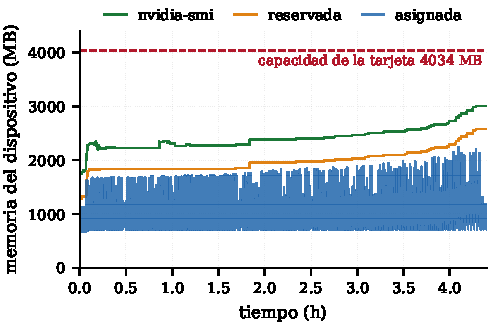
\includegraphics[width=\columnwidth]{figures/es/vram_trace.pdf}
\caption{Memoria del dispositivo a lo largo de la ejecución completa de 4\,h\,16\,min de
Qwen2.5-7B (114\,766 muestras cada 100\,ms). El diente de sierra es el \Cref{alg:usf} mismo: cada
diente es un ciclo $\textsc{Cargar}$--computar--$\textsc{Liberar}$ de una capa decodificadora de
0,43\,GB. El modelo ocupa 15,2\,GB en disco y, aun así, nada se aproxima a los 4034\,MB de la
tarjeta ---la imagen que el \Cref{thm:vram} predice. La deriva al alza de la curva reservada es el
asignador en caché reteniendo bloques liberados, no un crecimiento de lo que \usf{} mantiene
residente.}
\label{fig:vram}
\end{figure}

\begin{figure}[t]
\centering
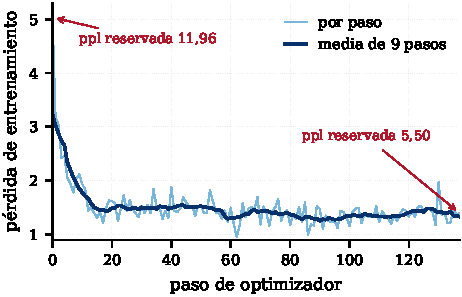
\includegraphics[width=\columnwidth]{figures/es/loss_curve.pdf}
\caption{Pérdida de entrenamiento a lo largo de 138 pasos de optimizador (275 micro-lotes con
$B{=}4$, $G{=}2$) sobre 1100 ejemplos de Alpaca. La perplejidad en datos reservados, medida sobre
100 ejemplos no vistos antes y después, cayó de 11,96 a 5,50. Ningún paso fue omitido por
desbordamiento de gradiente. Por el \Cref{thm:exact} esta trayectoria es la que habría producido
el entrenamiento ordinario con residencia: lo que la curva demuestra es que el sistema aprende;
qué tan bien lo hace queda fuera del alcance de este artículo.}
\label{fig:loss}
\end{figure}

\subsection{Layer-major}

La \Cref{tab:lm} compara ambas planificaciones sobre el modelo de 7\,B en 16 ejemplos con $G=4$.
Layer-major es $1{,}40\times$ más rápido y emplea \emph{menos} memoria, esto último porque sus
checkpoints residen en el anfitrión (\Cref{cor:depth}). La \eqref{eq:choiceG} predice mayores
ganancias con $G$ superior; no las medimos.

\begin{table}[t]
\centering
\caption{Batch-major frente a layer-major (Qwen2.5-7B, $B{=}4$, $S{=}256$, $G{=}4$, 16 ejemplos).}
\label{tab:lm}
\footnotesize
\begin{tabular}{@{}lrrr@{}}
\toprule
\textbf{Planificación} & \textbf{Total} & \textbf{Por ejemplo} & \textbf{VRAM pico} \\
\midrule
Batch-major & 457,5\,s & 28,6\,s & 2524\,MB \\
Layer-major & 327,4\,s & \textbf{20,5\,s} & \textbf{2219\,MB} \\
\midrule
Ganancia & \multicolumn{2}{c}{$\mathbf{1{,}40\times}$} & $-305$\,MB \\
\bottomrule
\end{tabular}
\end{table}

\subsection{Comparación con la cuantización}
\label{sec:quant}

La alternativa natural para reducir la memoria residente es la cuantización. En este presupuesto no
es meramente inferior: es inviable. Una cuantización NF4 a 4 bits de Qwen2.5-7B requiere 3,25\,GB
para los bloques transformer, más 1,09\,GB para la matriz de embeddings y otros 1,09\,GB para la
cabeza de modelado de lenguaje, que este modelo no ata al embedding y que la implementación de
referencia no cuantiza: 5,43\,GB frente a una tarjeta que expone 3,94\,GB. La predicción se
confirma ---la carga termina en un error de memoria agotada--- mientras que \usf{} entrena el mismo
modelo con un pico de 2,27\,GB en el asignador.

La comparación está trazada deliberadamente a favor de la cuantización. Los 5,43\,GB contabilizan
únicamente pesos, antes del estado del optimizador, las activaciones o el contexto CUDA, y son por
tanto una cota inferior de lo que 4 bits necesitaría; las cifras de \usf{} son tiempo de ejecución
medido y completo. La distancia es lo bastante amplia como para que la asimetría no altere nada, y
por eso podemos enunciar la conclusión como una separación de viabilidad y no como una
preferencia. Ambas técnicas son componibles y abordan ejes distintos: la cuantización compra
memoria con precisión, \usf{} la compra con tiempo, y solo esta última es exacta
(\Cref{cor:noapprox}).

%==============================================================================
\section{Análisis de Escalado}
\label{sec:scaling}

La \Cref{tab:claims} enuncia qué establece este artículo en cada escala y sobre qué base.

\begin{table}[t]
\centering
\caption{Alcance de las afirmaciones. Las tres filas poseen distinto estatus epistémico.}
\label{tab:claims}
\footnotesize
\begin{tabular}{@{}p{1.5cm}p{2.1cm}p{3.85cm}@{}}
\toprule
\textbf{Modelo} & \textbf{Estatus} & \textbf{Base} \\
\midrule
Qwen2.5-7B &
\textbf{Demostrado} &
Ejecutado: 2,2\,GB de pico, ppl $9{,}52\!\to\!4{,}46$, $\max|\Delta|=0$ \\[2pt]
Llama-3-70B &
\textbf{Predicho por la cota; no ejecutado} &
1,59\,GB por capa $<$ 3,94\,GB con una granularidad \emph{implementada}
(\Cref{tab:scaling}); no dispusimos de los pesos \\[2pt]
Llama-3-405B &
\textbf{Teórico; requiere una extensión no implementada} &
Precisa granularidad de matriz (1,62\,GB); véase la \Cref{rem:matrixlimit} \\
\bottomrule
\end{tabular}
\end{table}

Empleando~\eqref{eq:tio}--\eqref{eq:tcmp} con las constantes calibradas en la \Cref{sec:cost}, y
layer-major con $G=8$, el coste proyectado de 1000 ejemplos es de 4,0\,h para 7\,B, 41,7\,h para
70\,B y 245\,h para 405\,B; los tres están limitados por cómputo, de modo que las proyecciones las
gobierna $\Phi$ y no el ancho de banda de disco. La lectura honesta de estas cifras es que \usf{}
elimina la barrera de memoria y la sustituye por una barrera de tiempo. Un modelo de 70\,B pasa a
ser viable como demostración en una tarjeta de consumo; no pasa a ser un flujo de trabajo práctico.
El régimen práctico para esta clase de hardware es de 7\,B a 13\,B, y así lo hacemos constar en la
\Cref{sec:limits} en lugar de dejarlo a que el lector lo descubra.

%==============================================================================
\section{Limitaciones}
\label{sec:limits}

\textbf{El tiempo sustituye a la memoria.} \usf{} es sustancialmente más lento que el entrenamiento
residente; el método entero es un intercambio, y la \Cref{sec:scaling} lo cuantifica. Afirmamos
viabilidad en hardware donde la alternativa es no hacer nada en absoluto, no competitividad con una
GPU de centro de datos.

\textbf{Se requiere almacenamiento local.} El método presupone que los pesos están en un disco
local, y $\mathrm{BW}$ acota el término de E/S de~\eqref{eq:tio}.

\textbf{La hipótesis PEFT es estructural.} El \Cref{thm:vram} trata $|\theta|\cdot s_{\text{opt}}$
como pequeño. Con muchos parámetros entrenables, el estado del optimizador deja de ser
despreciable y su particionado pasa a ser la preocupación dominante, precisamente el régimen que
aborda ZeRO~\cite{rajbhandari2020zero}. \usf{} apunta a PEFT; el preentrenamiento queda fuera de
su alcance.

\textbf{La granularidad de matriz no está implementada} (\Cref{rem:matrixlimit}), razón por la cual
la \Cref{tab:claims} asigna a 405\,B un estatus más débil que a 70\,B.

\textbf{Las constantes son específicas del hardware.} El \emph{modelo} de coste de la
\Cref{sec:cost} es general; los valores de $\Phi$ y $\mathrm{BW}$ empleados en las
\Cref{tab:cost,tab:claims} no lo son, y requerirían recalibración en otro equipo.

\textbf{La inferencia no se ve afectada.} \usf{} es un método de entrenamiento.

%==============================================================================
\section{Conclusión}

Hemos mostrado que la memoria necesaria para ajustar un modelo de lenguaje congelado no es función
del tamaño del modelo. Es función de su unidad transmisible más grande, porque la diferenciación en
modo inverso es local: nada en la corrección ata un peso al dispositivo una vez computado su VJP,
así que cuánto tiempo permanece residente es algo que nos toca a nosotros planificar. El método
resultante es exacto ---verificado con desviación nula sobre el propio modelo de 7\,B---, agnóstico
al adaptador y gobernado por un modelo de coste preciso dentro de un 6\,\%.
Su consecuencia es un desplazamiento, y no una eliminación, del coste: el tamaño del modelo pasa a
ser una cuestión de tiempo y almacenamiento. En una GPU de consumo que un centro de datos
consideraría obsoleta, un modelo de 7\,B puede ahora ajustarse de forma exacta; la misma cota, con
una granularidad implementada, sitúa un modelo de 70\,B al alcance de esa misma tarjeta. La barrera
que queda es el tiempo, que la \Cref{sec:scaling} cuantifica y que ---a diferencia de la memoria---
no excluye a nadie de empezar.

\bibliographystyle{IEEEtran}
\bibliography{refs}

\end{document}